\subsection{Identifying Timing-flow Information Leaks}\label{sec:client-timingflow}

\begin{figure}[tp]
    \hfill
    \begin{subfigure}[b]{.5\textwidth}
        \begin{subfigure}{\linewidth}
            \centering
            \begin{chisel}
val dividend     = Input(UInt(32.W))
val divisor      = Input(UInt(32.W))
val quotient     = Reg(UInt(32.W))
val valid        = Reg(Bool())
// --- Simplified Design Logic ---
val reg_dividend = Reg(UInt(32.W))
val reg_divisor  = Reg(UInt(32.W))
when (reg_dividend >= reg_divisor) {
    reg_dividend := reg_dividend - reg_divisor
    quotient     := quotient + 1.U
} otherwise {
    valid        := true.B
}
            \end{chisel}
            \caption{A simplified Chisel example exhibiting a timing flow from the secret \texttt{divisor} to the observable \texttt{valid}.}
            \label{fig:timingflow-code}
        \end{subfigure}

        \vspace{1ex}

        \begin{subfigure}{\linewidth}
            \centering
            \footnotesize
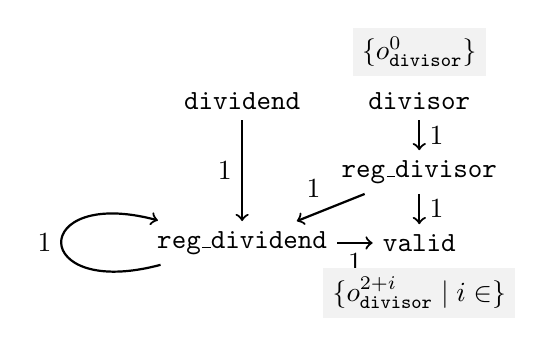
\begin{tikzpicture}[scale=.9,thick]
    \node (dd) at (0, 0) {$\textpurple{\mathtt{dividend}}$};
    \node (dr) at (2.5, 0) {$\textpurple{\mathtt{divisor}}$};

    \node (rdd) at (0, -2) {$\mathtt{reg\_dividend}$};
    \node (rdr) at (2.5, -1) {$\mathtt{reg\_divisor}$};
    \node (v)  at (2.5, -2) {$\mathtt{valid}$};

    \draw[->] (dd) -- node[left]{$1$} (rdd);
    \draw[->] (rdd) edge[loop left] node{$1$} (rdd);
    \draw[->] (rdr) -- node[above left]{$1$} (rdd);
    \draw[->] (rdd) -- node[below]{$1$} (v);

    \draw[->] (dr) -- node[right]{$1$} (rdr);
    \draw[->] (rdr) -- node[right]{$1$} (v);

    \node[fill=gray!10] at (2.5, .7) {$\{o_{\mathtt{divisor}}^0\}$};
    \node[fill=gray!10] at (2.5, -2.7) {$\{o_{\mathtt{divisor}}^{2+i}\mid i\in\nats\}$};
\end{tikzpicture}

            \caption{\tia results showing various temporal influences from the secret \texttt{divisor} to the observable \texttt{valid}.}
            \label{fig:tia-timingflow}
        \end{subfigure}


    \end{subfigure}
    \hfill
    \begin{subfigure}[b]{.46\textwidth}
        \begin{subfigure}{\linewidth}
            \centering
            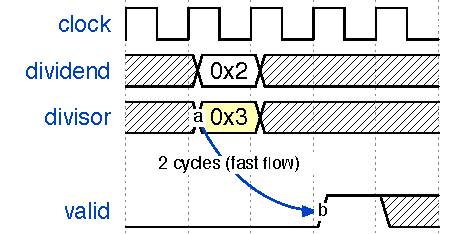
\includegraphics[width=\linewidth,clip,trim=10 0 10 0]{figures/timingflow-fast-waveform}
            \caption{Waveform illustrating a \emph{fast} flow from \texttt{divisor} to \texttt{valid}.}
            \label{fig:timingflow-waveform-fast}
        \end{subfigure}

        \vspace{1ex}

        \begin{subfigure}{\linewidth}
            \centering
            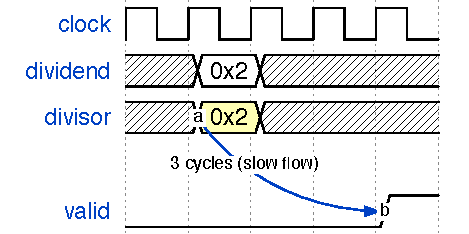
\includegraphics[width=\linewidth,clip,trim=10 0 10 0]{figures/timingflow-slow-waveform}
            \caption{Waveform illustrating a \emph{slow} flow from \texttt{divisor} to \texttt{valid}.}
            \label{fig:timingflow-waveform-slow}
        \end{subfigure}

        \vspace{1ex}

        \begin{subfigure}{\linewidth}
            \centering
            \[
            \left|\left\{o_{\mathtt{divisor}}^i \in \absT(\mathtt{valid})\right\}\right| > 1
            \]
            \caption{An observation guiding timing flow analysis.}
            \label{fig:timingflow-observe}
        \end{subfigure}
    \end{subfigure}
    \hfill
    \caption{A motivating example for timing-flow analysis.}
\end{figure}

A \emph{timing flow} is a form of implicit information flow in which sensitive information affects the timing of public hardware behavior, potentially enabling information leakage~\cite{hu_hardware_2022,ardeshiricham_clepsydra_2017,qin_formal_2020}.
We first illustrate timing flows through a simplified example and then describe how our timing-flow analysis detects them leveraging the fundamental temporal influence information provided by \tia.

\paragraph{Example of A Timing Flow}

Figure~\ref{fig:timingflow-code} shows a simplified Chisel example exhibiting the timing flow described by~\cite{ardeshiricham_clepsydra_2017}.
The circuit computes \texttt{quotient} (Line~3) from the given \texttt{dividend} (Line~1) and \texttt{divisor} (Line~2) using consecutive subtraction (Lines~6--13), with \texttt{valid} (Line~4) indicating when the computation has completed.
For simplicity, we omit the initialization logic that takes one cycle to load \texttt{dividend} into \texttt{reg\_dividend}, \texttt{divisor} into \texttt{reg\_divisor}, and reset \texttt{valid} to \texttt{false}.
Figures~\ref{fig:timingflow-waveform-fast} and~\ref{fig:timingflow-waveform-slow} illustrate how different values of \texttt{divisor} can cause \texttt{valid} to be asserted at different times, thereby creating a timing flow from \texttt{divisor}\footnote{A similar timing flow exists from \texttt{dividend} to \texttt{valid}; we focus on \texttt{divisor} for simplicity.} to \texttt{valid}.
For a fixed \texttt{dividend = 2}, consider two possible values of \texttt{divisor}.
When \texttt{divisor = 3}, the computation completes after two cycles: the first cycle initializes the registers, and the second cycle evaluates Line~8 as false and asserts \texttt{valid} at Line~12.
This corresponds to the \emph{fast} flow shown in Figure~\ref{fig:timingflow-waveform-fast}.
In contrast, when \texttt{divisor = 2}, Line~8 evaluates to true in the second cycle, causing one subtraction at Lines~9--10.
The computation therefore requires an additional cycle before \texttt{valid} is asserted by Line~12, resulting in the \emph{slow} flow shown in Figure~\ref{fig:timingflow-waveform-slow}.

Next we'll describe how such a timing flow from \texttt{divisor} to \texttt{dividend} can lead to information leak.
Consider a security scenario in which the design is open source, \texttt{dividend} is public, and \texttt{divisor} is a secret key.
Suppose an attacker cannot observe the computed \texttt{quotient}, but can measure the number of clock cycles between providing the inputs and observing \texttt{valid}.
For the slow-flow case, the attacker observes three cycles: one initialization cycle, one subtraction cycle, and one cycle in which \texttt{valid} is asserted.
Because the algorithm is known, the attacker can therefore infer that
\[
\mathtt{divisor} \leq \mathtt{dividend}
< 2\cdot\mathtt{divisor},
\]
which, for $\mathtt{dividend}=2$, implies $\mathtt{divisor}=2$.
For the fast-flow case, the attacker can at least infer that $\mathtt{divisor} > \mathtt{dividend}$.
Thus, the timing of \texttt{valid} reveals information about the secret \texttt{divisor}.
If \texttt{valid} were asserted after the same number of cycles for every possible \texttt{divisor}, no such timing-based leakage would occur.

\paragraph{Insights of Timing-flow Analysis}

Figure~\ref{fig:tia-timingflow} shows the \tia results for the circuit in Figure~\ref{fig:timingflow-code}, focusing on how \texttt{divisor} temporally influences \texttt{valid}.
We can observe that \texttt{divisor} can influence \texttt{valid} after multiple distinct numbers of clock cycles.
These distinct temporal influences correspond to the different timing behaviors illustrated in Figures~\ref{fig:timingflow-waveform-fast} and~\ref{fig:timingflow-waveform-slow}, providing an indication of the timing flow from \texttt{divisor} to \texttt{valid}.
This observation is summarized in Figure~\ref{fig:timingflow-observe}.

Guided by this observation, we generalize \texttt{divisor} to an arbitrary secret source signal $p\in\ports$ and \texttt{valid} to an arbitrary observable sink signal $x\in\variables$.
Our \emph{timing-flow analysis} reports a timing flow from $p$ to $x$ if
\[
\left|\left\{o_p^i \in \absT(x)\right\}\right| > 1,
\]
where $\absT$ is the temporal influence information computed by \tia.
Intuitively, this criterion identifies whether the same source can affect the sink after more than one number of clock cycles, indicating that the source may influence the timing of the sink.
